\documentclass[8pt,oneside]{extbook}

%\usepackage{subfigure}
\usepackage{subcaption}
\usepackage{tabularx}
\usepackage{graphicx}
\usepackage{amsmath}
\usepackage{amsfonts}
\usepackage{hyperref}
\usepackage{adjustbox}
\usepackage{listings}
\usepackage{optidef}
\usepackage{cleveref}
\usepackage{threeparttable}
\usepackage{xcolor}
\usepackage{titlesec}
\usepackage{enumitem}
\usepackage{mathrsfs}
\usepackage[gen]{eurosym}
\usepackage[driver=pdftex]{geometry}
\usepackage{import}
\usepackage{tabu}
%\usepackage{titleformat{\section
%        {\normalfont\normalzie\bfseries}{Helo.}{1em}{}


\definecolor{codegreen}{rgb}{0,0.6,0}
\definecolor{codegray}{rgb}{0.5,0.5,0.5}
\definecolor{codepurple}{rgb}{0.58,0,0.82}
\definecolor{backcolour}{rgb}{0.95,0.95,0.92}

\crefname{table}{table}{table}
\setlength{\parindent}{0em}
\setlength{\parskip}{0.7em}

%\counterwithin{table}{section}
 
\lstdefinestyle{mystyle}{
    backgroundcolor=\color{backcolour},   
    commentstyle=\color{codegreen},
    keywordstyle=\color{magenta},
    numberstyle=\tiny\color{codegray},
    stringstyle=\color{codepurple},
    basicstyle=\ttfamily\footnotesize,
    breakatwhitespace=false,         
    breaklines=true,                 
    captionpos=b,                    
    keepspaces=true,                 
    numbers=left,                    
    numbersep=5pt,                  
    showspaces=false,                
    showstringspaces=false,
    showtabs=false,                  
    tabsize=2
}

\newlist{syms}{itemize}{1}
\setlist[syms,1]{label=,labelwidth=0.25in,align=parleft,itemsep=0.1\baselineskip,leftmargin=!}

\newtheorem{theorem}{Theorem}
\newtheorem{definition}{Definition}
\newtheorem{proof}{Proof}
 
\lstset{style=mystyle}

%\usepackage[margin=0.5in]{geometry}
\usepackage{inputenc}

\newcommand{\Real}{\mathbb{R}}
\newcommand{\Int}{\mathbb{Z}}
\newcommand{\Nat}{\mathbb{N}}
\newcommand{\Complex}{\mathbb{C}}
\newcommand{\vect}[1]{\boldsymbol{#1}}

%\renewcommand{\TPTminimum}{\textwidth}

\renewcommand{\Re}[1]{\mathfrak{Re}\left\lbrace{#1}\right\rbrace}
\renewcommand{\Im}[1]{\mathfrak{Im}\left\lbrace{#1}\right\rbrace}

%\DeclareMathOperator*{\minimize}{minimize}
%\DeclareMathOperator*{\maximize}{maximize}

%\title{{\bf MATH 3172 3.0\\ Combinatorial Optimization}\\\vspace{10pt} \large Final Exam
%    \author{Jacques Nel}
%}

\title{{\bf LE/EECS 3172 3.0\\ Combinatorial Optimization}\\\vspace{10pt} \large Final Exam
    \author{Jacques Nel}
}

\begin{document}

\maketitle

\thispagestyle{empty}

\newpage

\pagenumbering{arabic}

\chapter{B-2 Construction of a stadium}

A town council wishes to construct a small stadium in order to improve the
services provided to the people living in the district. After the invitation to
tender, a local construction company is awarded the contract and wishes
to complete the task within the shortest possible time. All major tasks are
listed in the following table. The durations are expressed in weeks. Some tasks
can only start after the completion of certain other tasks. The last two
columns of the table refer to question 2 which we shall see later.

\textbf{Question 1:} What is the earliest possible date of completing the
construction?

\textbf{Question 2:} The town council would like the project to terminate earlier
than the time announced by the builder (answer to question 1). To obtain this,
the council is prepared to pay a bonus of $\euro{}30\mathrm{K}$ for every week the work
finishes early. The builder needs to employ additional workers and rent more
equipment to cut down on the total time. In the preceding table he has 
summarized the maximum number of weeks he can save per task (column "Max. reduct.")
and the associated additional cost per week. When will the project be completed
if the builder wishes to maximize his profit?

\newpage

\section{Question 1}

\subsection{Parameters}

\begin{syms}
\item[$T$] enumerates $n=18+1$ project tasks, ie. $T=\left\lbrace 1,\ldots, n+1\right\rbrace$

\item[$A$] the matrix of arcs with $A\in\left\lbrace 0,1\right\rbrace^{n+1\times n+1}$;
    with elements $a_{ij}=\begin{cases}1 & \texttt{task } j \text{ preceeds }\texttt{task }i\\
    0 & \text{otherwise}\end{cases}$

\item[$d_t$] the duration in weeks to complete task $t\in T$ with no additional labour hours allocated

\end{syms}

\textbf{Note:} A ficticious task \texttt{Done} with $t=19$ and $d_{19}=0$ is also added which has all other
terminal tasks as predecessors.

\subsubsection{Data given for parameters}

\begin{table}[h]
    \center
    \caption{Data for stadium construction}\label{table:1-1}
    {\small
    \begin{tabu}{clcccc}
        \hline
        \rowfont[c]{\bfseries} Task & Description & Duration $d_t$ & Predecessors $P_t$ & Max. reduct. $r_t$ & Add. cost $c_t$ \\
        \hline
        {\bfseries 1} & Installing the construction site & 2 & - & 0 & - \\
        {\bfseries 2} & Terracing  & 16 & 1 & 3 & 30 \\
        {\bfseries 3} & Constructing the foundations & 9 & 2 & 1 & 26 \\
        {\bfseries 4} & Access roads and other networks  & 8 & 2 & 2 & 12 \\
        {\bfseries 5} & Erecting the basement  & 10 & 3 & 2 & 17 \\        
        {\bfseries 6} & Main floor  & 6 & 4, 5 & 1 & 15 \\
        {\bfseries 7} & Dividing up the changing rooms  & 2 & 4 & 1 & 8 \\
        {\bfseries 8} & Electrifying the terraces  & 2 & 6 & 0 & - \\
        {\bfseries 9} & Constructing the roof  & 9 & 4, 6 & 2 & 42 \\
        {\bfseries 10} & Lighting of the stadium  & 5 & 4 & 1 & 21 \\
        {\bfseries 11} & Installing the terraces  & 3 & 6 & 1 & 18 \\
        {\bfseries 12} & Sealing the roof  & 2 & 9 & 0 & - \\
        {\bfseries 13} & Finishing the changing rooms  & 1 & 7 & 0 & - \\
        {\bfseries 14} & Constructing the ticket office  & 7 & 2 & 2 & 22 \\
        {\bfseries 15} & Secondary access roads  & 4 & 4, 14 & 2 & 12 \\
        {\bfseries 16} & Means of signalling  & 3 & 8, 11, 14 & 1 & 6 \\
        {\bfseries 17} & Lawn and sport acessories  & 9 & 12 & 3 & 16 \\
        {\bfseries 18} & Handing over the building  & 1 & 17 & 0 & - \\
        \hline
                       &\\
    \end{tabu}
}
    \emph{Note:} Columns $r_t$ and $c_t$ is not used for question 1.
\end{table}

\newpage

\subsubsection{Task precedence}

Some task $t\in T$ may have a predecessor $p\in T$. In other words task $t$ can not
commence until task $p$ is finished. In this example, ``Erecting the basement'' can
not be begun until after ``Constructing the foundation'' completes.

For some task $t\in T$, it has predecessors as the set 
$P_t = \left\lbrace p_{t0}, \ldots, p_{tk} : p_{tk} \in T \text{ and }
    p_{tk} \text{ preceeds } p_{t0} \right\rbrace$. Note that we could have
    $P_t = \emptyset$. One may visualize this graph as in \cref{figure:1-1}.


\begin{figure}[h]
    \center
    \caption{Graph of precedence dependencies of tasks}\label{figure:1-1}
    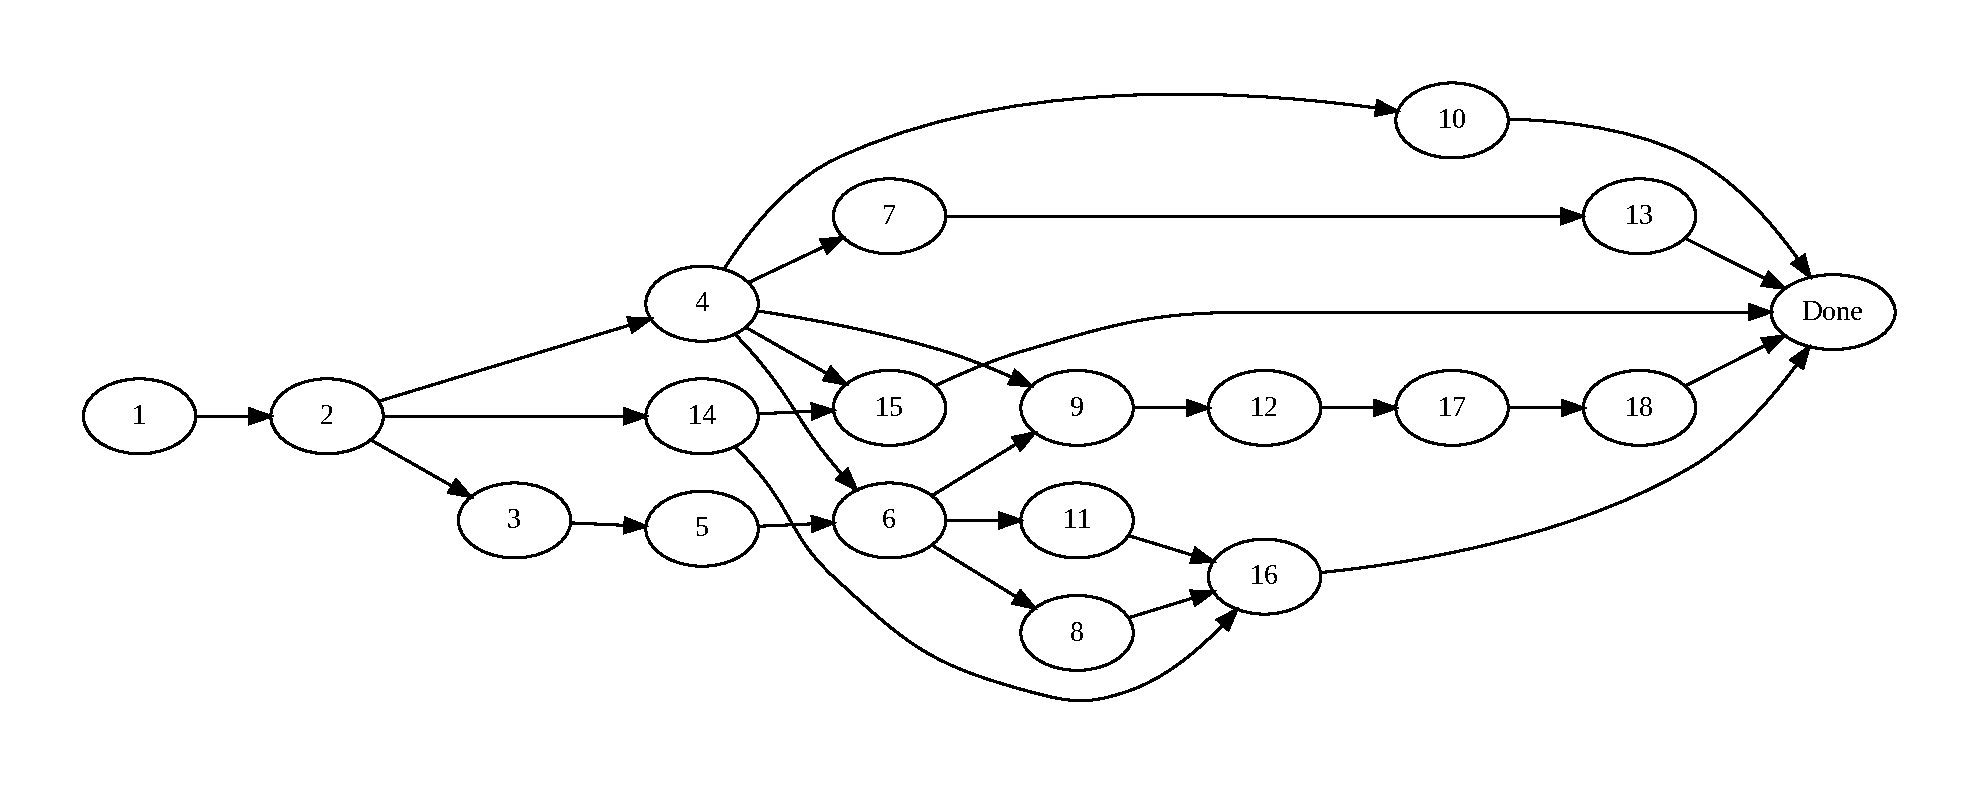
\includegraphics[width=14cm,keepaspectratio]{../figures/fig1-1}
\end{figure}

\subsection{Decision variable}

\begin{syms}
\item[$x_t$] indicates the week in which task $t\in T$ starts; $0 \leq x_t\in \Int$. For convience
    let $\vect{x} = \left( x_1, \ldots, x_t\right)^T \in \Int^n$.
\end{syms}

\subsection{Model}


\begin{mini!}
    {\vect{x}}{f\left(x_{n+1}\right)=x_{n+1} \protect\label{eq:b2-q1-obj}}{\label{eq:b2-q1}}{}
    \addConstraint{x_i}{\geq a_{ij}( x_j + d_j), \forall (i, j) \in T\times T \protect\label{eq:b2-q1-ctr1}}
    \addConstraint{x_t}{\geq 0, \forall t \in T \protect\label{eq:b2-q1-ctr2}}
\end{mini!}

The objective $f(x_{n+1})$ given by \cref{eq:b2-q1-obj} is the start time of task
with $t=19$. Since $d_{19}=0$, this also is the end time of the final task. In other
words, we week to minimize the time of completion of the entire project.

\Cref{eq:b2-q1-ctr1} simply enforces that task $i$, which starts at $x_i$ can not 
start until its predecessor $j$, which finishes at week $x_j+d_j$, is complete.
When there is no arc from $j$ to $i$, $a_{ij}=0$ and the inequality constraint is
satisfied. \Cref{eq:b2-q1-ctr1} is the canonical non-negativity constraint on $\vect{x}$.

\subsection{Results}\label{section:1.1.4}

\newpage

\section{Question 2}

\subsection{Parameters}

\begin{syms}
    \item[$T$] enumerates $n=18+1$ project tasks, ie. $T=\left\lbrace 1,\ldots,n+1\right\rbrace$

    \item[$A$] the matrix of arcs with $A\in\left\lbrace 0,1\right\rbrace^{n+1\times n+1}$;
    with elements $a_{ij}=\begin{cases}1 & \texttt{task } j \text{ preceeds }\texttt{task }i\\
    0 & \text{otherwise}\end{cases}$

    \item[$d_t$] the duration in weeks to complete task $t\in T$ with no additional labour hours allocated

    \item[$r_t$] the maximum reduction in duration of task $t\in T$ in weeks that can be 
        achieved by allocating additional labour

    \item[$c_t$] cost in $1000\euro{}$ / week when allocating additional labour
        to task $t\in T$.

    \item[$b$] bonus paid in $1000\euro{}$ per week the project finishes early; 
        with $b=30$

\end{syms}

Refer to \cref{table:1-1} for values of the above parameters.

\subsection{Decision variables}

\begin{syms}
\item[$x_t$] indicates the week in which task $t\in T$ starts; $0 \leq x_t\in \Int$. For convience
    let $\vect{x} = \left( x_1, \ldots, x_{n+1}\right)^T \in \Int^{n+1}$.

\item [$y_t$] indicates the number of weeks by which duration of task $t\in T$ is
    reduced; with $0\leq y_t \in\Int$. For convience, let
    $\vect{y} = \left( y_1,\ldots, y_n\right)^T \in \Int^n$
\end{syms}

\subsection{Model}


\begin{maxi!}
    {\vect{x}, \vect{y}}{g\left(\vect{x}, \vect{y}\right)=b\left(x_{n+1}-f_1^\star\right) \protect\label{eq:b2-q2-obj}}{\label{eq:b2-q2}}{}
    \addConstraint{x_i}{\geq a_{ij}( x_j + d_j - y_j), \forall (i, j) \in T\times T \protect\label{eq:b2-q2-ctr1}}
    \addConstraint{y_t}{\leq r_t, \forall t\in T\setminus \left(n+1\right) \protect\label{eq:b2-q2-ctr2}}
    \addConstraint{x_t}{\geq 0, \forall t\in T \protect\label{eq:b2-q2-ctr3}}
    \addConstraint{y_t}{\geq 0, \forall t\in T \protect\label{eq:b2-q2-ctr4}}
\end{maxi!}

Let $f^*$ be the optimal value of the objective function found in results for 
question 1 in \cref{section:1.1.4}, ie. the earliest time which the project can
be completed without allocating additional labour. The completion date which
maximizes the bonus paid to the countractor is given by:

$$
y_{n+1} = x_{n+1} - f_1^\star.
$$

Then the total bonus for completing the job early is given by

\begin{equation}\label{eq:b2-q2-obj1}
g\left(\vect{x}, \vect{y}\right) = b y_{n+1} = b\left(x_{n+1}-f_1^*\right).
\end{equation}

The above \cref{eq:b2-q2-obj1} is the quantity that the contractor seeks to maximize and becomes 
the objective function \cref{eq:b2-q2-obj}. \Cref{eq:b2-q2-ctr1} is similar to 
\cref{eq:b2-q1-ctr1}, in \cref{section:1.1.4}, but takes into account the reduction in duration
for the previous task. The maximum possible reduction in duration for task
$t\in T$ is limited by $r_t$. This is represented by the family of constraints
in \cref{eq:b2-q2-ctr2}. \Cref{eq:b2-q2-ctr3} and \cref{eq:b2-q2-ctr4} are simply
the family of canonical non-negativity constraints on decision variables
$\vect{x}$ and $\vect{y}$.

\subsection{Results}

\chapter{D-1 Wagon load balancing}

Three railyay wagons with a carrying capacity of 100 quintals (1 quintal = 100 kg)
have been reserved to transport sixteen boxes. The weight of the boxes in quintals
is given in the following table. How shall the boxes be assigned to the wagons
in order to keep to the limits on the maximum carrying capacity and to
minimize the heaviest wagon load?

\section{Parameters}

\begin{syms}

\item[$B$] enumerates $m=16$ boxes; ie. $B=\left\lbrace 1,\ldots, m\right\rbrace$

\item[$W$] enumerates $n=3$ railway wagons; ie. $W=\left\lbrace 1,\ldots, n\right\rbrace$

\item[$c$] denotes maximum capacity of a wagon in quintals, with $c=100$

\item[$\mu_b$] denotes the weight of box $b\in B$

\end{syms}

Refer to \cref{table:2-1} for the values of the above parameters.

\begin{table}[h]
    \center
    \caption{Weight of boxes}\label{table:2-1}
    \begin{tabu}{lcccccccc}
        \hline
        \rowfont[lcccccccc]{\bfseries} Box & 1 & 2 & 3 & 4 & 5 & 6 & 7 & 8 \\
        \textbf{Weight} & 34 & 6 & 8 & 17 & 16 & 5 & 13 & 21 \\
        \hline
        \rowfont[lcccccccc]{\bfseries} Box & 9 & 10 & 11 & 12 & 13 & 14 & 15 & 16 \\
        \textbf{Weight} & 25 & 31 & 14 & 13 & 33 & 9 & 25 & 25 \\
        \hline

    \end{tabu}
\end{table}

\section{Decision variable}

\begin{syms}

\item[$x_{bw}$] indicates box $b\in B$ is loaded in wagon $w\in W$; 
    $x_{bw}\in \left\lbrace 0, 1\right\rbrace$. For convience let
    $\vect{x} \in \left\lbrace 0, 1\right\rbrace^{m\times n}$
    with entries $x_{bw}, \forall (b,w) \in B\times W$.

\item[$m$] ancillary variable denoting upper bound of weights in
    quintals of all wagons;
    $0\leq m\in\Int$
\end{syms}

\section{Model}

\begin{mini!}
    {\vect{x}}{f(m)=m \protect\label{eq:d1-obj}}{\label{eq:d1}}{}
    \addConstraint{\sum_{w\in W}x_{bw}}{= 1, \forall b \in B \protect\label{eq:d1-ctr1}}
    \addConstraint{m}{\geq \sum_{b\in B}\mu_b x_{bw}, \forall w \in W \protect\label{eq:d1-ctr2}}
    \addConstraint{\sum_{b\in B}\mu_b x_{bw}}{\leq c, \forall w\in W\protect\label{eq:d1-ctr3}}
    \addConstraint{x_{bw}}{\in\left\lbrace 0, 1\right\rbrace, \forall \left(b,w\right)\in B\times W\protect\label{eq:d1-ctr4}}
    \addConstraint{m}{\geq 0 \protect\label{eq:d1-ctr5}}
\end{mini!}

The objective we week to minimize \cref{eq:d1-obj} is simply $m$ or rather,
the upper bound on the weights of each wagon $w\in W$. Each box $b\in B$ must
be loaded in exactly one wagon $w\in W$ as stated by \cref{eq:d1-ctr1}. 

For
$m$ to be the least upper bound of the weights of each wagon $w\in W$,
$m$ must be greater than all wagon weights as expressed in \cref{eq:d1-ctr2}. Minimization will lower it until
it is equal to the maximum of the weights of the loaded wagons. Note that this
objective is wrong in the text.

\Cref{eq:d1-ctr4} enforces that the decision variable $\vect{x}$ is a binary indicator,
and \cref{eq:d1-ctr5} is the canonical non-negativity constraint on $m$.

\section{Results}

\chapter{D-3 Tank loading}

Five tanker ships have arrived at a chemical factory. They are carrying loads
of liquid products that must not be mixed. Refer to \cref{table:arrive} for
these quantities. Nine tanks of different capacities are available on site.
Some of them are already partially filled with a liquid. \Cref{table:tanks}
lists the characteristics of the tanks (in tonnes). Into which tanks should
the ships be unloaded (question 1) to maximize the capacity of the tanks
that remain unused, or (question 2) to maximize the number of tanks that remain
free?

\section{Question 1}

\subsection{Parameters}

\begin{syms}

\item[$T$] enumerates the $n=9$ tanks, ie. $T=\left\lbrace 1,\ldots,n\right\rbrace$

\item[$L$] enumerates the $m=5$ types of liquid arriving at the facility:
    $\left\lbrace \texttt{Benzol},\texttt{Butanol},\texttt{Propanol},
    \texttt{Styrene}, \texttt{THF}\right\rbrace$ ie.
    $L=\left\lbrace 1,\ldots, m\right\rbrace$.

\item[$F$] the indices of the prefilled tanks, ie. 
    $\left\lbrace \texttt{Benzol}, \texttt{THF}\right\rbrace$
    with $F = \left\lbrace T\in L : \text{tank } t \text{ is prefilled}\right\rbrace \subset T$

\item[$a_l$] denotes the amount (in tonnes) of liquid $l\in L$ arriving at the
    facility

\item[$c_t$] denotes the capacity (in tonnes) of tank $t\in T$

\item[$Q_t$] denotes the innitial amount (in tonnes) of liquid in tank $t\in F$

\item[$P_t$] denotes the type of liquid initially in tank $t\in F$

\item[$R_l$] remainder of liquid $l\in L$ after filling prefilled tanks $t\in F$ 
    to capacity with liquid of same type, given by


\begin{equation}
    R_l = \begin{cases}\displaystyle
        a_l - \sum_{t\in F\text, P_t = l} c_t - Q_t & \text{if }t\in F\\
        a_l & \text{otherwise}
    \end{cases}
\end{equation}

\end{syms}
    
Refer to \cref{table:arrive} for the values of $a_l$ and \cref{table:tanks} for
the values of $F, c_t, Q_t$, and $P_t$.

\begin{table}
    \center
    \caption{Various types of liquid arriving at facility}\label{table:arrive}
    \begin{tabu}{lcccccc}
        \hline
        \rowfont[lcccccc]{\bfseries} Type & Benzol & Butanol & Propanol & Styrene & THF \\
        \hline
        \textbf{Qauntity (in tonnes)} $a_l$ & 1200 & 700 & 1000 & 450 & 1200 \\
        \hline
    \end{tabu}
\end{table}

\begin{table}
    \center
    \caption{Facillity tank capacities and innitial quantities}\label{table:tanks}
    \begin{tabu}{lccccccccc}
        \hline
        \rowfont[lccccccccc]{\bfseries} Tank & 1 & 2 & 3 & 4 & 5 & 6 & 7 & 8 & 9\\
        \hline
        \textbf{Capacity (tonnes)} $c_t$ & 500 & 400 & 400 & 600 & 600 & 900 & 800 & 800 & 800 \\
        \textbf{Initial type} $Q_t$ & - & \texttt{Benzol} & - & - & - & - & \texttt{THF} & - & - \\
        \textbf{Initial amount (tonnes)} $P_t$ & 0 & 100 & 0 & 0 & 0 & 0 & 300 & 0 & 0 \\
        \hline
    \end{tabu}
\end{table}


\subsection{Decision variable}

\begin{syms}

\item[$x_{lt}$] indicates that remaining liquid of type $l\in L$ is pumped into
    tank $t\in T$, after prefilling; for convience let 
    $\vect{x}\in\left\lbrace 0, 1\right\rbrace^{m\times n}$ with entries $x_{lt}$

\end{syms}
\subsection{Model} \label{section:3.1.3}

\begin{mini!}
    {\vect{x}}{f(\vect{x})=\sum_{l\in L}\sum_{t\in T\setminus F} c_t x_{lt} \protect\label{eq:d3-q1-obj}}{\label{eq:d3-q1}}{}
    \addConstraint{\sum_{t\in T\setminus F} c_t x_{lt}}{& \geq R_l, \forall l\in L \protect\label{eq:d3-q1-ctr1}}
    \addConstraint{\sum_{l\in L}x_{lt}}{& \leq 1, \forall t\in T\setminus F \protect\label{eq:d3-q1-ctr2}}
    \addConstraint{x_{lt}}{& \in \left\lbrace 0, 1\right\rbrace, \forall (l,t)\in L\times T \protect\label{eq:d3-q1-ctr3}}
\end{mini!}

Maximizing the remaining capacity is equivalent to minmizing the used capacity
in a tank as expressed in \cref{eq:d3-q1-obj}. The family of constraints
\cref{eq:d3-q1-ctr1} ensures that all remaining liquid, after prefilling, is pumped
into tanks for all liquids $l\in L$. Liquids of different types can not be
allowed to mix in a tank. This is guaranteed by \cref{eq:d3-q1-ctr2}.
Lastly, \cref{eq:d3-q1-ctr3} states that $\vect{x}$ must be a binary variable.

\subsection{Results}

\section{Question 2}

We approach question 2 in almost an identical way as in question 1. The only thing
that changes is the objective function. The model for question 2 is given
below.

\subsection{Model}

\begin{mini!}
    {\vect{x}}{g(\vect{x})=\sum_{l\in L}\sum_{t\in T\setminus F} x_{lt} \protect\label{eq:d3-q2-obj}}{\label{eq:d3-q2}}{}
    \addConstraint{\sum_{t\in T\setminus F} c_t x_{lt}}{& \geq R_l, \forall l\in L \protect\label{eq:d3-q2-ctr1}}
    \addConstraint{\sum_{l\in L}x_{lt}}{& \leq 1, \forall t\in T\setminus F \protect\label{eq:d3-q2-ctr2}}
    \addConstraint{x_{lt}}{& \in \left\lbrace 0, 1\right\rbrace, \forall (l,t)\in L\times T \protect\label{eq:d3-q2-ctr3}}
\end{mini!}

\Cref{eq:d3-q2-obj} is similar to \cref{eq:d3-q1-obj} in \cref{section:3.1.3}.
The only difference between $g(\vect{x})$ and $f(\vect{x})$ is that $g\vect{x})$
does not include the tank capacities $c_t$. The result is, we are only counting
the number of tanks that used. Once again, minimizing this quantity is clearly
equivalent to maximizing the number of unused tanks.

\subsection{Results}

\chapter{E-1 Car rental}

A small car rental company has a fleet of 94 vechiles distributed among its
10 agencies. The location of every agency is given by its geographical coordinates
$X$ and $Y$ in a grid based on kilometers. We assume that the road distance
between agencies is approximately 1.3 times the Euclidean distance. Refer to
\cref{table:coords} for the geographical coordinates of all agencies, the inventory
of cars required the next morning, and the inventory of cars in the evening
preceeding this day. Refer to \cref{table:car-stock} for the available and required
inventories of the various agencies.

Suppose the cost for transporting a car is $\euro{}0.50$ per km, determine the
movements of cars that allow the company to re-establish the required numbers of
cars at all agencies, minimizing the total cost incurred for transport.

\section{Parameters}

\begin{syms}

\item[$A$] enumerates $n=10$ rental agencies, ie. $A=\left\lbrace 1,\ldots, n\right\rbrace$

\item[$\vect{X}_a$] denotes the geographical coordinates of an agency $a\in A$, with
    $\vect{X}_a \in \Real^2$, for convience let $\vect{X} \in \Real^{2\times n}$ with
    columns $\vect{X}_a, \forall a\in A$

\item[$r_a$] number of cars required by agency $a\in A$ on next morning

\item[$s_a$] number of cars agency $a\in A$ has in the evening

\item[$E$] part of the partition of $A$ with 
    $E= \left\lbrace a\in A : s_a > r_a \right\rbrace \subset A$

\item[$N$] part of the parition of $A$ with
    $N = \left\lbrace a\in A: s_a < r_a \right\rbrace \subset A$

\item[$c$] transporation cost in \euro{} / km, with $c=\euro{}0.50$ / km

\item[$\lambda$] Euclidean distance to road distance multiplier, with $\lambda=1.3$

\end{syms}

\begin{table}[h]
    \center
    \caption{Geographical coordinates of agencies}\label{table:coords}
    \begin{tabu}{lcccccccccc}
        \hline
        \rowfont[lcccccccccc]{\bfseries} Agency $a$ & 1 & 2 & 3 & 4 & 5 & 6 & 7 & 8 & 9 & 10\\
        \hline
        \textbf{X coordinate (km grid)} $X_a^{(x)}$ & 0 & 20 & 18 & 30 & 35 & 33 & 5 & 5 & 11 & 2 \\
        \textbf{Y coordinate (km grid)} $X_a^{(y)}$ & 0 & 20 & 10 & 12 & 0 & 25 & 27 & 10 & 0 & 15 \\
        \hline
    \end{tabu}
\end{table}

\begin{table}[h]
    \center
    \caption{Available and required inventory of agencies}\label{table:car-stock}
    \begin{tabu}{lcccccccccc}
        \hline
        \rowfont[lcccccccccc]{\bfseries} Agency $a$ & 1 & 2 & 3 & 4 & 5 & 6 & 7 & 8 & 9 & 10\\
        \hline
        \textbf{Cars present} $s_a$ & 8 & 13 & 4 & 8 & 12 & 2 & 14 & 11 & 15 & 7 \\
        \textbf{Cars required} $r_a$ & 10 & 6 & 8 & 11 & 9 & 7 & 15 & 7 & 9 & 12 \\
        \hline
    \end{tabu}
\end{table}

\section{Decision variable}

\begin{syms}

    \item[$x_{ij}$] denotes the number of cars transpored from an agency
        with excess $i\in E$ to an agency with shortage $j\in N$;
        $0 \leq x_{ij} \in \Int$; for convience let $\vect{x} \in \Int^{|E|\times|N|}$
        with entries $x_{ij}$

\end{syms}

\section{Model}

\begin{mini!}
    {\vect{x}}{f(\vect{x})=\sum_{i\in E}\sum_{j\in N} c \lambda x_{ij} \sqrt{\vect{X}_i - \vect{X}_j} \protect\label{eq:e1-obj}}{\label{eq:e1}}{}
    \addConstraint{\sum_{i\in E} x_{ij}}{& = s_j - r_j, \forall j\in N \protect\label{eq:e1-ctr1}}
    \addConstraint{\sum_{j\in N} x_{ij}}{& = s_i - r_i, \forall i\in N \protect\label{eq:e1-ctr2}}
    \addConstraint{x_{ij}}{& \geq 0, \forall (i,j) \in E\times N \protect\label{eq:e1-ctr3}}
\end{mini!}


\section{Results}

\chapter{E-5 Combining different modes of transport}

A load of 20 tonnes needs to be transported on a rouate passing through five cities,
with a choice of three different modes of transport: rail, road, and air. In any
of the three intermediate cities it is possible to change the mode of transport
but the load uses a single mode of transport between two consecutive cities.
Refer to \cref{table:transport-costs} for the cost of the various modes of
transport between pairs of cities.

Furthermore, changing the mode of tranport incurs an associated cost. This cost
is indepdependent of location. Refer to \cref{table:transfer-costs} for these
costs.

How should we organize the transport of the load at the least cost?

\section{Parameters}

\begin{syms}

\item[$M$] enumerates the $n=3$ modes of transport:
    $\left\lbrace \texttt{rail}, \texttt{road}, \texttt{air}\right\rbrace$,
    with $M=\left\lbrace 1, \ldots, n\right\rbrace$

\item[$L$] enumerates the $k=5$ legs of the route between the cities, ie.
    $L=\left\lbrace 1,\ldots, k\right\rbrace$

\item[$c_{ml}$] denotes the transportation cost per tonne on leg $l\in L$ of the route
    using mode $m\in M$

\item[$t_{ij}$] denotes the cost per tonne of transfering the cargo from mode $i\in M$ to mode
    $j\in M$ at a given city

\item[$q$] denotes the weight of the cargo in tonnes with $q=20$ tonnes

\end{syms}

Refer to \cref{table:transport-costs} for values of $c_{ml}$ and to \cref{table:transfer-costs}
for values of $t_{ij}$.

\begin{table}[h]
    \center
    \caption{Transportation costs between pairs of cities using various modes of transport}
    \label{table:transport-costs}
    \begin{tabu}{lcccc}
        \hline
        \rowfont[lcccc]{\bfseries} & 1-2 & 2-3 & 3-4 & 4-5 \\
        \hline
        \textbf{Rail} & 30 & 25 & 40 & 60 \\
        \textbf{Road} & 25 & 40 & 45 & 50 \\
        \textbf{Air} & 40 & 20 & 50 & 45 \\
        \hline
    \end{tabu}
\end{table}

\begin{table}[h]
    \center
    \caption{Costs of changing mode of transport}\label{table:transfer-costs}
    \begin{tabu}{lccc}
        \hline
        \rowfont[lccc]{\bfseries} from/to & Rail & Road & Air \\
        \hline
        \textbf{Rail} & 0 & 5 & 12 \\
        \textbf{Road} & 8 & 0 & 10 \\
        \textbf{Air} & 15 & 10 & 0 \\
        \hline
    \end{tabu}
\end{table}

\section{Decision variables}

\begin{syms}

\item[$x_{ml}$] indicates that mode $m\in M$ is used on leg $l\in L$ of the route;
    $x_{ml} \in \left\lbrace 0, 1\right\rbrace$; for convenience, let
    $\vect{x} \in \left\lbrace 0, 1\right\rbrace^{n\times k}$ with entries
    $x_{ml}$

\item[$y_{ijl}$] indicates whether cargo is transfered from mode $i\in M$ to mode
    $j\in M$ after leg $l\in L$ of the journey; $y_{ijl}\in\left\lbrace 0, 1\right\rbrace$;
    for convenience, we define the tensor 
    $\vect{y} \in\left\lbrace 0, 1\right\rbrace^{n\times n\times k}$

\end{syms}

\section{Model}

The total tranportation cost is given by

\begin{equation}
    g(\vect{x}) = \sum_{m\in M}\sum_{l\in l} c_{ml} x_{ml}.
\end{equation}

The total cost of transfering the cargo between modes of transportation
is

\begin{equation}
    h(\vect{y}) = \sum_{i\in M}\sum_{j\in M}\sum_{l\in L\setminus \left\lbrace k\right\rbrace}
    t_{ij}y_{ijl}
\end{equation}

\begin{mini!}
    {\vect{x}}{f(\vect{x},\vect{y})=g(\vect{x}) +h(\vect{y}) \protect\label{eq:e5-obj}}{\label{eq:e5}}{}
    \addConstraint{\sum_{m\in M}x_{ml}}{& = 1, \forall l\in L \protect\label{eq:e5-ctr1}}
    \addConstraint{\sum_{i, j\in M} y_{ijl}}{& = 1, \forall l\in L\setminus\left\lbrace k\right\rbrace \protect\label{eq:e5-ctr2}}
    \addConstraint{x_{il}}{& \geq y_{ijl}, \forall i, j \in M, l\in L\setminus\left\lbrace k\right\rbrace \protect\label{eq:e5-ctr3}}
    \addConstraint{x_{ml}}{& \in \left\lbrace 0, 1\right\rbrace, \forall m\in M, l\in L \protect\label{eq:e5-ctr4}}
    \addConstraint{y_{ijl}}{& \in \left\lbrace 0, 1\right\rbrace, \forall i,j \in M, l\in L \protect\label{eq:e5-ctr5}}
\end{mini!}

\section{Results}

\chapter{F-4 Airline hub location}

The airline FAL (French Air Lines) sepcializes in freight transport. The company
links the major French cities with cities in the United States,
nameley Atlanta, Boston, Chicago, Marseille, Nice, and Paris. The average
quantities in tonnes transported every day by this company between these cities
are given in \cref{table:f4-quant}.

We shall assume that the transport cost between two cities $i$ and $j$
is proportional to the distance that seperates them. The distances in miles
are given in \cref{table:f4-dist}.

The airline is planning to use two cities as connection paltforms
(\textbf{hubs}) to reduce the transport costs. Every city is then assigned a single
hub. The traffic between cities assigned to a given hub $H_1$ to the cities
assigned to the other hub $H_2$ is all routed through the single connection
form $H_1$ to $H_2$ which allows the airline to reduce the transport cost
by 20\%. Determine the two cities to be chosen as hubs in order to minimize
the transport cost.

\section{Parameters}

\begin{syms}

\item[$C$] enumerates $m=5$ cities: 
$\left\lbrace \texttt{Atlanta}, \texttt{Boston}, \texttt{Chicago}, \texttt{Marseille}, \texttt{Nice}\right\rbrace$,
ie. $C=\left\lbrace 1, \ldots, n\right\rbrace$

\item[$n$] denotes the number of hubs to choose, with $n=2$
    
\item[$q_{ij}$] denotes the average quantity of goods in tonnes transported between city
    $i\in C$ and $j\in C$ in a given day

\item[$d_{ij}$] denotes the distance from city $i\in C$ to city $j\in C$

%\item[$f_{ij}$] is the non-reduced transportation cost from city $i\in C$ to city $j\in C$

\item[$c_{ijkl}$] is proportional to the transportation cost from city $i\in C$ to city $j\in C$ through
    hubs $k\in C$ and $l\in C$

\item[$r$] is the reduced hub to hub transport cost factor, with $r=0.8$

\end{syms}

$c_{ijkl}$ is calculated from $d_{ij}$ and $r$ as follows:

\begin{equation}
    c_{ijkl} = d_{ik} + rd_{kl} + d_{lj}, \forall i,j,k,l \in C
\end{equation}

\emph{Note:} When any one of the two suscripts are equal, we have $d_{ii}=0$.

\begin{table}
    \center
    \caption{Average daily quantities of freight in tonnes}\label{table:f4-quant}
    \begin{tabu}{lcccccc}
        \hline
        \rowfont[lcccccc]{\bfseries} & Atlanta & Boston & Chicago & Marseille & Nice & Paris \\
        \hline
        \textbf{Atlanta} & 0 & 500 & 1000 & 300 & 400 & 1500 \\
        \textbf{Boston} & 1500 & 0 & 250 & 630 & 360 & 1140 \\
        \textbf{Chicago} & 400 & 510 & 0 & 460 & 320 & 490 \\
        \textbf{Marseille} & 300 & 600 & 810 & 0 & 820 & 310 \\
        \textbf{Nice} & 400 & 100 & 420 & 730 & 0 & 970 \\
        \textbf{Paris} & 350 & 1020 & 260 & 580 & 380 & 0 \\
        \hline
    \end{tabu}
\end{table}

\begin{table}
    \center
    \caption{Distances between pairs of cities in miles}\label{table:f4-dist}
    \begin{tabu}{lccccc}
        \hline
        \rowfont[lccccc]{\bfseries} & Boston & Chicago & Marseille & Nice & Paris \\
        \hline
        \textbf{Atlanta} & 945 & 605 & 4667 & 4749 & 4394 \\
        \textbf{Boston} & & 866 & 3726 & 3806 & 3448 \\
        \textbf{Chicago} & & & 4471 & 4541 & 4152 \\
        \textbf{Marseille} & & & & 109 & 415 \\
        \textbf{Nice} & & & & & 431 \\
        \hline
    \end{tabu}
\end{table}

\newpage

\section{Decision variables}

\begin{syms}

\item[$x_{ijkl}$] indicates that the cargo flows from city $i\in C$ to city
    $j\in C$ via hubs $k\in C$ and $l\in C$, in other words

    $x_{ijkl} = \begin{cases}1 & \text{cargo flows from city }i\text{ to }j\text{ via hub }k\text{ to }l \\
        0 & \text{otherwise}
    \end{cases}$,

    for convenience, define the tensor $\vect{x} \in \left\lbrace 0, 1\right\rbrace^{n\times n\times n\times n}$
    with entries $x_{ijkl}$

\item[$y_i$] indicates whether city $i\in C$ is a hub, in other words

        $y_i = \begin{cases}1 & \text{city }i\text{ is a hub} \\
            0 & \text{otherwise}
        \end{cases}$,

    for convenience, define the tuple $\vect{y} = \left( y_1,\ldots, y_n\right) \in \left\lbrace 0, 1\right\rbrace^n$


\end{syms}

\section{Model}

\begin{mini!}
    {\vect{x}}{f(\vect{x})=\mathop{\sum\sum\sum\sum}_{i,j,k,l\in C} c_{ijkl} c_{ijkl}q_{ij}x_{ijkl} \protect\label{eq:f4-obj}}{\label{eq:f4}}{}
    \addConstraint{\sum_{i\in C} y_i}{= n \protect\label{eq:f4-ctr1}}
    \addConstraint{\mathop{\sum\sum}_{k,l\in C} x_{ijkl}}{= 1, \forall i, j\in C \protect\label{eq:f4-ctr-2}}
    \addConstraint{x_{ijkl}}{\leq y_{k}, \forall i,j, k, l \in C \protect\label{eq:f4-ctr-3}}
    \addConstraint{x_{ijkl}}{\leq y_{l}, \forall i,j, k, l \in C \protect\label{eq:f4-ctr-4}}
    \addConstraint{x_{ijkl}}{\in \left\lbrace 0, 1\right\rbrace, \forall i,j,k,l \in C \protect\label{eq:f4-ctr-5}}
    \addConstraint{y_i}{\in \left\lbrace 0, 1\right\rbrace, \forall i\in C \protect\label{eq:f4-ctr-6}}
\end{mini!}
\section{Results}



\end{document}
